\chapter{Results}
\label{sec:results}

%FLOATING POTENTIAL SUMMARY
% \begin{table}[]
% \centering
% \begin{tabular}{cccccc}
% \hline
% & No photoelectron & Drift along Z & Drift along X & External Magnetic Field & Photoelectron temperature 3 eV\\\hline
% With booms & N/A & 105.419 & 105.400 & 105.400 & 78.154\\\hline
% Without booms & N/A & 100.710 & 100.696 & 100.699 & N/A\\\hline
% \end{tabular}
% \caption{Dummy text}
% \label{tab:FlotingPotSummary}
% \end{table}



\section{Charging without photoemission}
%FLOATING POTENTIAL CONVERGENCE
%POTENTIAL THROUGH CENTER OF OBJECT
%PARTICLE DENSITIES (rho_i and rho_e)
%RHO_I
%RHO_E
%AVERAGE POTENTIAL ISOLINES XY


\section{Charging with photoemission}

\subsection*{Drift parallel to X axis}

%FLOATING POTENTIAL CONVERGENCE
\begin{figure}[H]
  \centering
  \begin{subfigure}[b]{0.75\textwidth}
  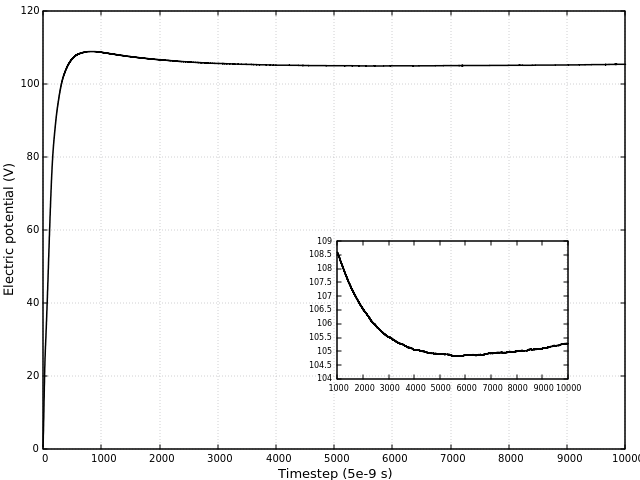
\includegraphics[width=\columnwidth]{figures/MMO/posX/WB/C_posX_WB.png}
  \caption{Booms}
  \label{fig:C_posX_WB}
\end{subfigure}
\hfill
\begin{subfigure}[b]{0.75\textwidth}
  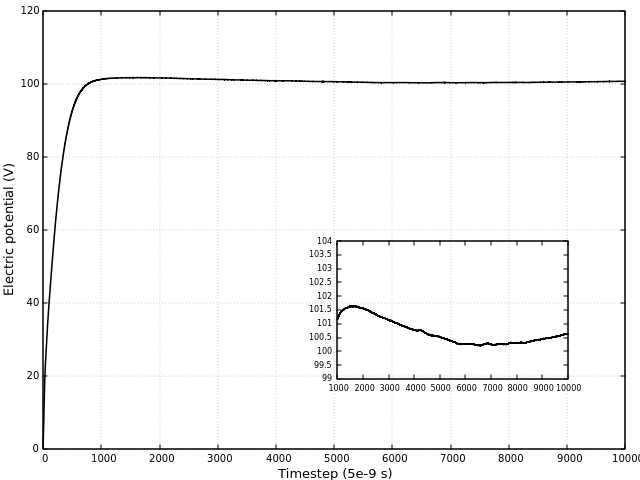
\includegraphics[width=\columnwidth]{figures/MMO/posX/NB/C_posX_NB.png}
  \caption{Without booms}
  \label{fig:C_posX_NB}
\end{subfigure}
\label{fig:Conv_posX}
\caption{Time series plot of the potential of the MMO with and without booms. The inset plots the same timeseries after 1000 timesteps, where the potential of the spacecraft has begun to oscillate about the floating potential.}
\end{figure}


%POTENTIAL THROUGH CENTER OF OBJECT

\begin{figure}[H]
  \begin{subfigure}[b]{0.6\textwidth}
  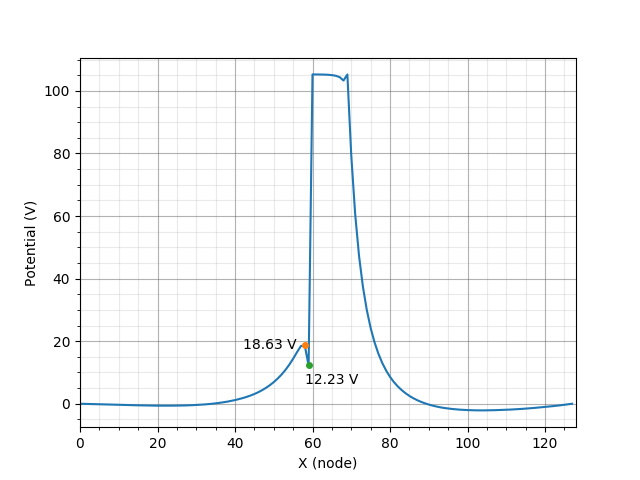
\includegraphics[width=\textwidth]{figures/MMO/posX/WB/L_posX_WB.png}
  \caption{Booms}
  \label{fig:L_posX_WB}
\end{subfigure}
\begin{subfigure}[b]{0.6\textwidth}
  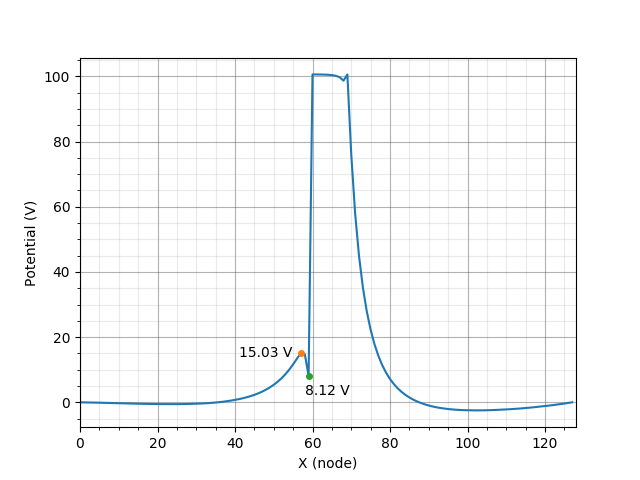
\includegraphics[width=\textwidth]{figures/MMO/posX/NB/L_posX_NB.png}
  \caption{Without booms}
  \label{fig:L_posX_NB}
\end{subfigure}
\label{fig:Line_posX}
\caption{Dummy text}
\end{figure}


%AVERAGE POTENTIAL ISOLINES XY

\begin{figure}[H]
  \begin{subfigure}[b]{0.6\textwidth}
    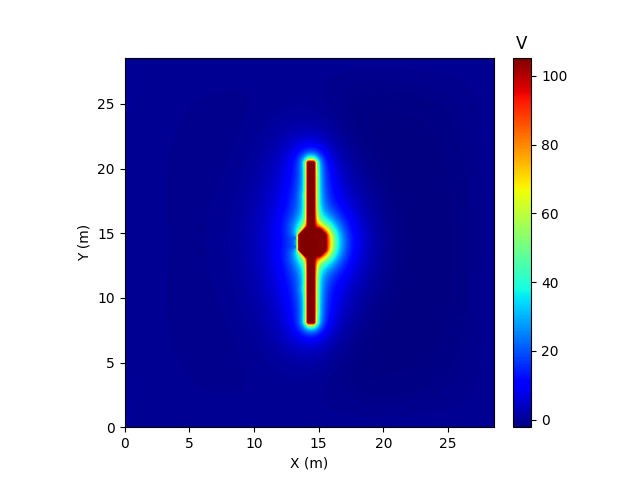
\includegraphics[width=\textwidth]{figures/MMO/posX/WB/P_posX_WB.png}
    \caption{Booms}
    \label{fig:P_posX_WB}
  \end{subfigure}
  \begin{subfigure}[b]{0.6\textwidth}
    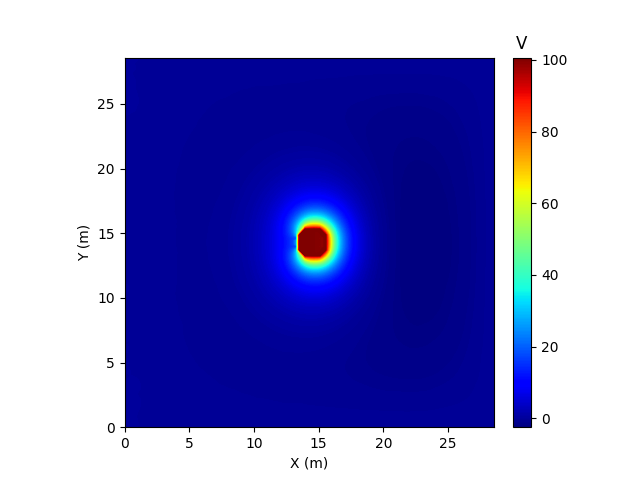
\includegraphics[width=\textwidth]{figures/MMO/posX/NB/P_posX_NB.png}
    \caption{Without booms}
    \label{fig:P_posX_NB}
  \end{subfigure}
  \label{fig:Pot_posX}
  \caption{Dummy text}
\end{figure}



%PARTICLE DENSITIES (rho_i and rho_e)
%RHO_I

\begin{figure}[H]
  \begin{subfigure}[b]{0.6\textwidth}
  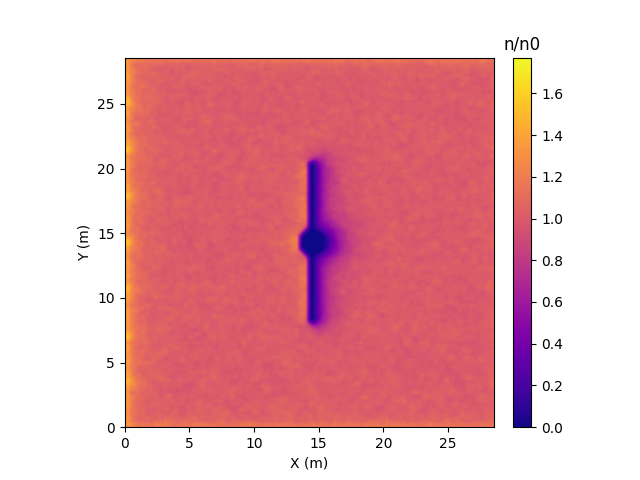
\includegraphics[width=\textwidth]{figures/MMO/posX/WB/I_posX_WB.png}
  \caption{Booms}
  \label{fig:I_posX_WB}
  \end{subfigure}
\begin{subfigure}[b]{0.6\textwidth}
  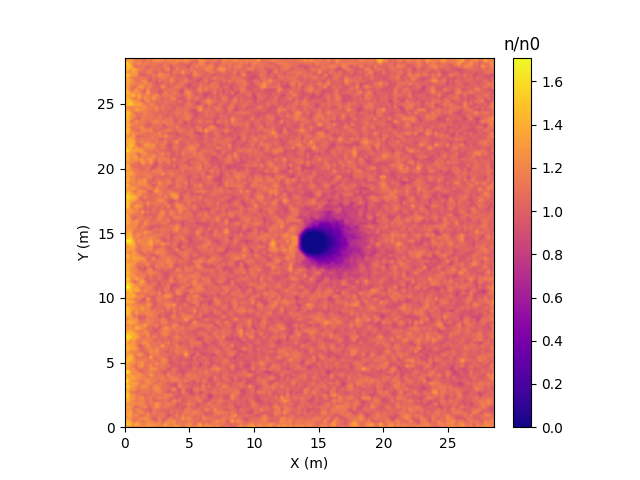
\includegraphics[width=\textwidth]{figures/MMO/posX/NB/I_posX_NB.png}
  \caption{Without booms}
  \label{fig:I_posX_NB}
\end{subfigure}
\label{fig:Ions_posX}
\caption{Dummy text}
\end{figure}


%RHO_E

\begin{figure}[H]
  \begin{subfigure}[b]{0.6\textwidth}
  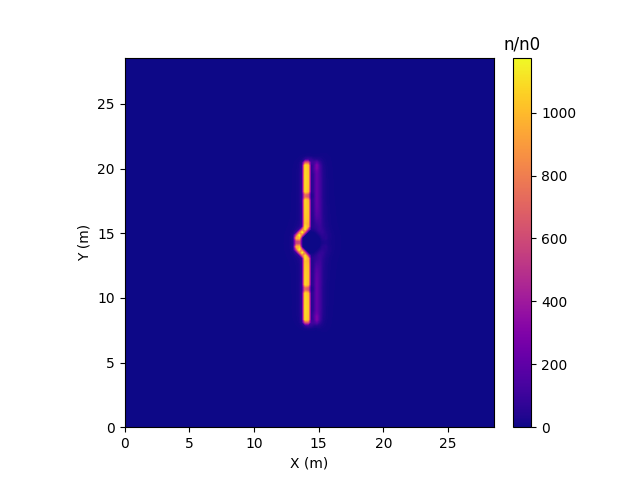
\includegraphics[width=\textwidth]{figures/MMO/posX/WB/E_posX_WB.png}
  \caption{Booms}
  \label{fig:E_posX_WB}
\end{subfigure}
\begin{subfigure}[b]{0.6\textwidth}
  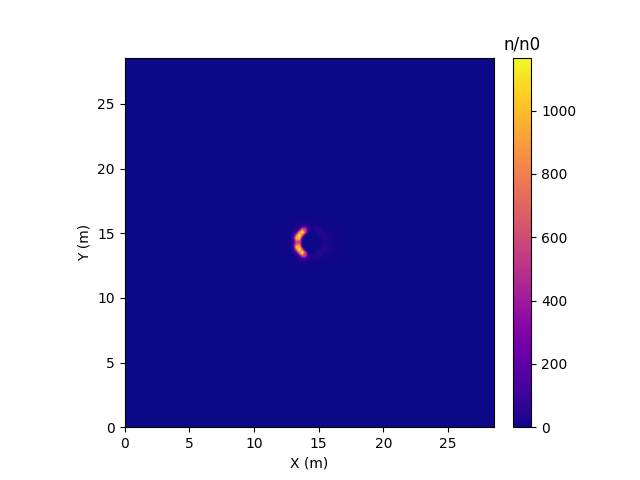
\includegraphics[width=\textwidth]{figures/MMO/posX/NB/E_posX_NB.png}
  \caption{Without booms}
  \label{fig:E_posX_NB}
\end{subfigure}
\label{fig:Elec_posX}
\caption{Dummy text}
\end{figure}




\subsection*{Drift parallel to Z axis}
%FLOATING POTENTIAL CONVERGENCE

\begin{figure}[H]
  \centering
  \begin{subfigure}[b]{0.75\textwidth}
  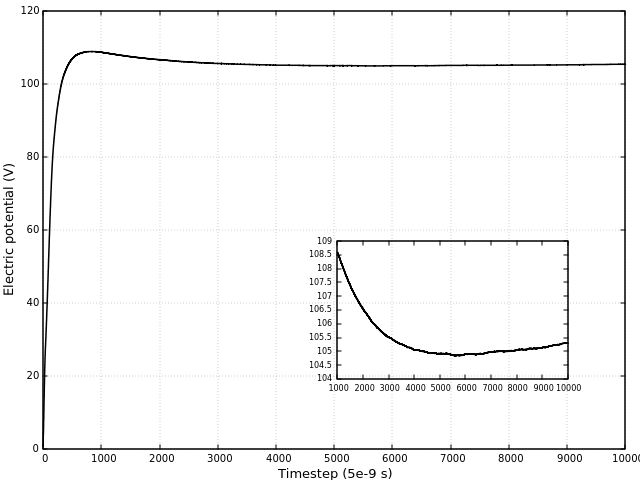
\includegraphics[width=\columnwidth]{figures/MMO/minZ/WB/C_minZ_WB.png}
  \caption{Booms}
  \label{fig:C_minZ_WB}
\end{subfigure}
\par\bigskip
\begin{subfigure}[b]{0.75\textwidth}
  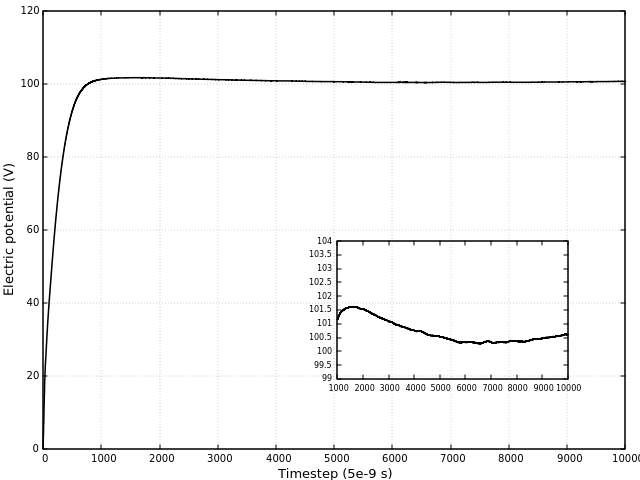
\includegraphics[width=\columnwidth]{figures/MMO/minZ/NB/C_minZ_NB.png}
  \caption{Without booms}
  \label{fig:C_minZ_NB}
\end{subfigure}
\label{fig:Conv_minZ}
\caption{Time series plot of the potential of the MMO with and without booms. Where the drift is along the negative Z axis. The inset plots the same timeseries after 1000 timesteps, where the potential of the spacecraft has begun to oscillate about the floating potential.}
\end{figure}


%POTENTIAL THROUGH CENTER OF OBJECT

\begin{figure}[H]
  \begin{subfigure}[b]{0.6\textwidth}
  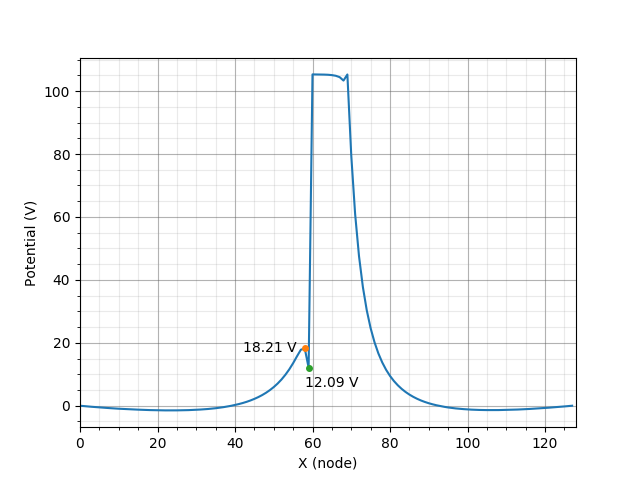
\includegraphics[width=\textwidth]{figures/MMO/minZ/WB/L_minZ_WB.png}
  \caption{Booms}
  \label{fig:L_minZ_WB}
\end{subfigure}
\begin{subfigure}[b]{0.6\textwidth}
  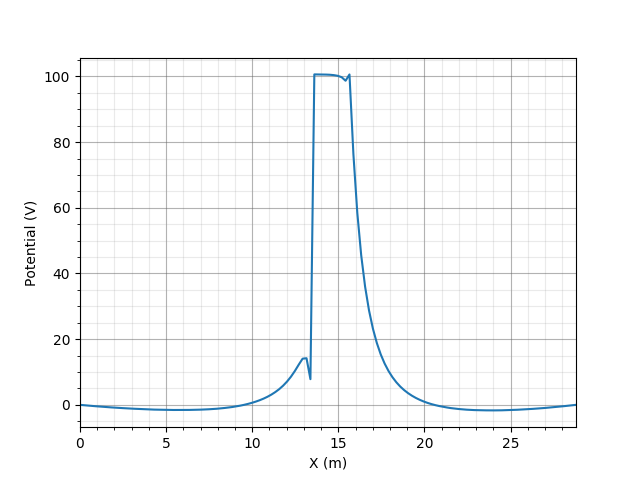
\includegraphics[width=\textwidth]{figures/MMO/minZ/NB/L_minZ_NB.png}
  \caption{Without booms}
  \label{fig:L_minZ_N}
\end{subfigure}
\label{fig:Line_minZ}
\caption{Dummy text}
\end{figure}


%AVERAGE POTENTIAL ISOLINES XY
\begin{figure}[H]
  \begin{subfigure}[b]{0.6\textwidth}
    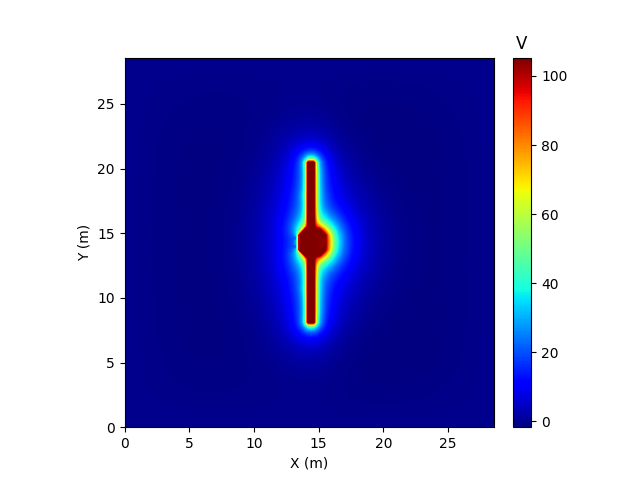
\includegraphics[width=\textwidth]{figures/MMO/minZ/WB/P_minZ_WB.png}
    \caption{Booms}
    \label{fig:P_minZ_WB}
  \end{subfigure}
  \hfill
  \begin{subfigure}[b]{0.6\textwidth}
    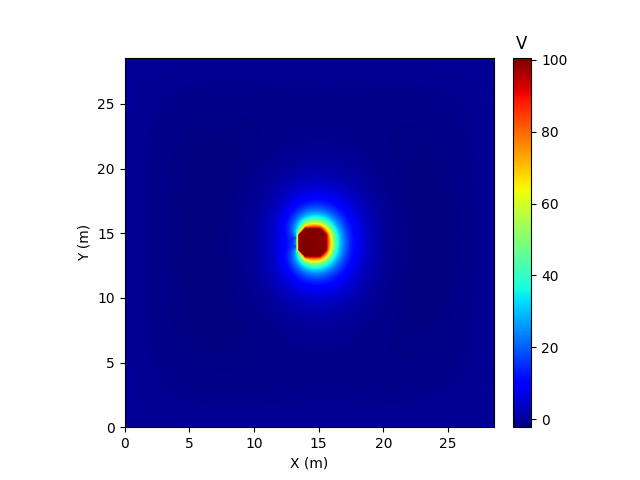
\includegraphics[width=\textwidth]{figures/MMO/minZ/NB/P_minZ_NB.png}
    \caption{Without booms}
    \label{fig:P_minZ_NB}
  \end{subfigure}
  \label{fig:Pot_minZ}
  \caption{Dummy text}
\end{figure}

%PARTICLE DENSITIES (rho_i and rho_e)
%RHO_I
\begin{figure}[H]
  \begin{subfigure}[b]{0.6\textwidth}
  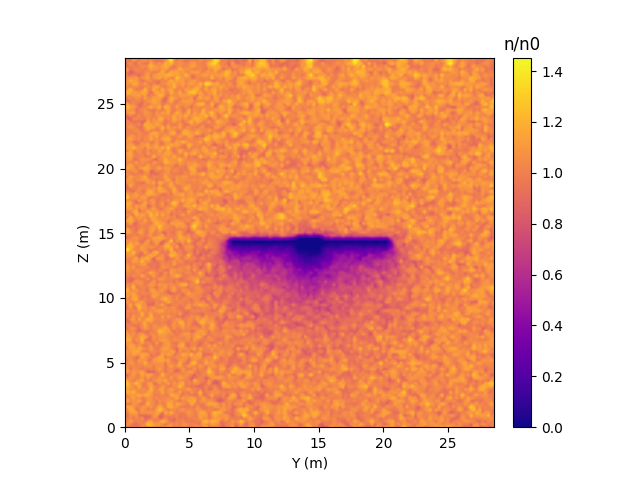
\includegraphics[width=\textwidth]{figures/MMO/minZ/WB/I_minZ_WB.png}
  \caption{Booms}
  \label{fig:I_minZ_WB}
\end{subfigure}
\begin{subfigure}[b]{0.6\textwidth}
  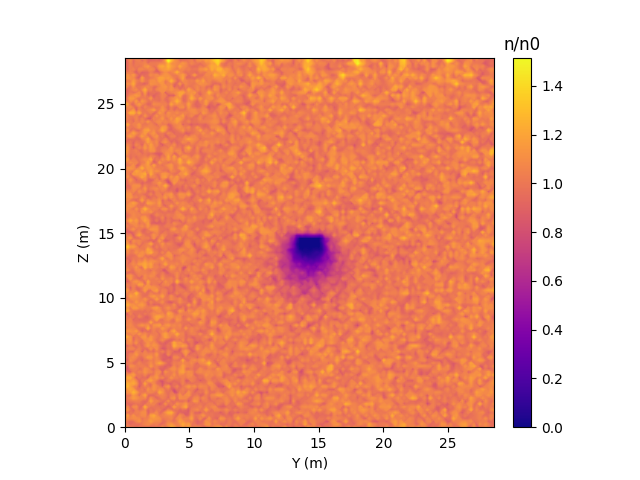
\includegraphics[width=\textwidth]{figures/MMO/minZ/NB/I_minZ_NB.png}
  \caption{Without booms}
  \label{fig:I_minZ_NB}
\end{subfigure}
\label{fig:Ion_minZ}
\caption{Dummy text}
\end{figure}

%RHO_E
\begin{figure}[H]
  \begin{subfigure}[b]{0.6\textwidth}
  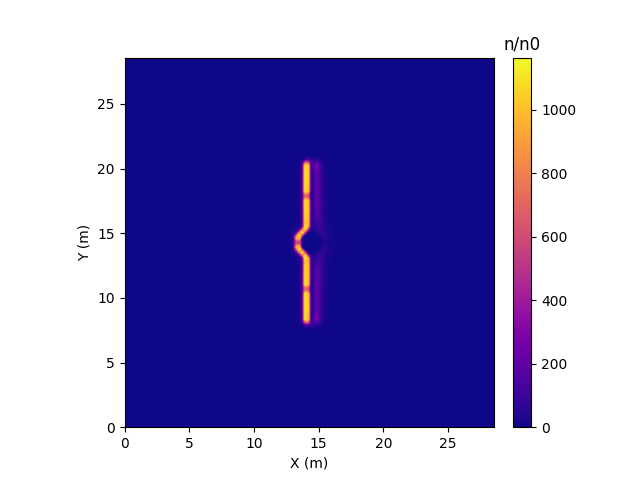
\includegraphics[width=\textwidth]{figures/MMO/minZ/WB/E_minZ_WB.png}
  \caption{Booms}
  \label{fig:E_minZ_WB}
\end{subfigure}
\begin{subfigure}[b]{0.6\textwidth}
  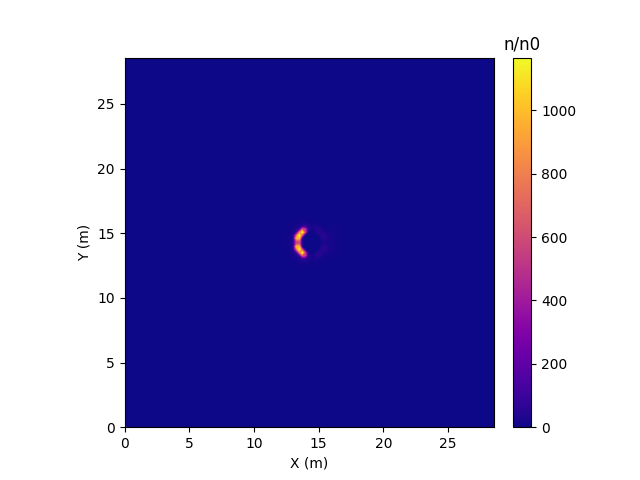
\includegraphics[width=\textwidth]{figures/MMO/minZ/NB/E_minZ_NB.png}
  \caption{Without booms}
  \label{fig:E_minZ_NB}
\end{subfigure}
\label{fig:Elec_minZ}
\caption{Dummy text}
\end{figure}


\section{Charging in an external magnetic field}

%FLOATING POTENTIAL CONVERGENCE
\begin{figure}[H]
  \begin{subfigure}[b]{0.75\textwidth}
  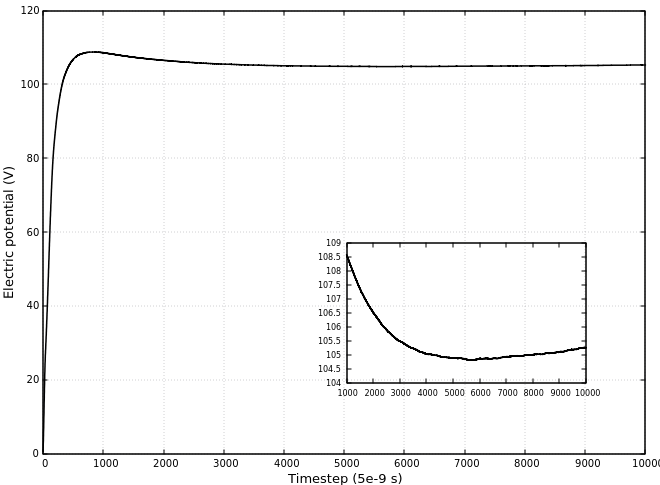
\includegraphics[width=\columnwidth]{figures/MMO/BField/WB/C_BField_WB.png}
  \caption{Booms}
  \label{fig:C_BField_WB}
\end{subfigure}
\par\bigskip
\begin{subfigure}[b]{0.75\textwidth}
  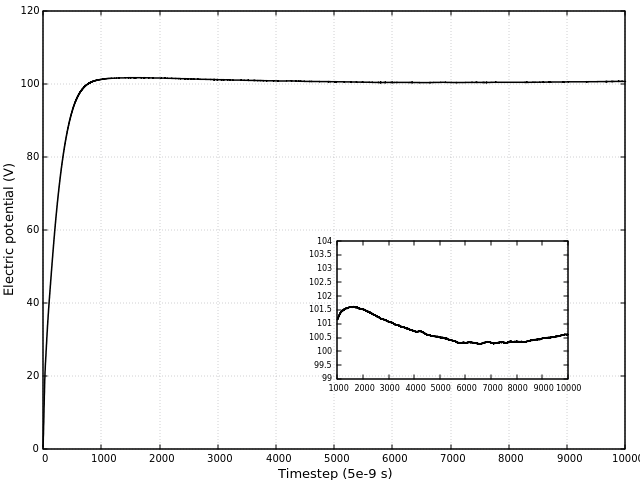
\includegraphics[width=\columnwidth]{figures/MMO/BField/NB/C_BField_NB.png}
  \caption{Without booms}
  \label{fig:C_BField_NB}
\end{subfigure}
\label{fig:Conv_BField}
\caption{Dummy text}
\end{figure}


%POTENTIAL THROUGH CENTER OF OBJECT

\begin{figure}[H]
  \begin{subfigure}[b]{0.6\textwidth}
  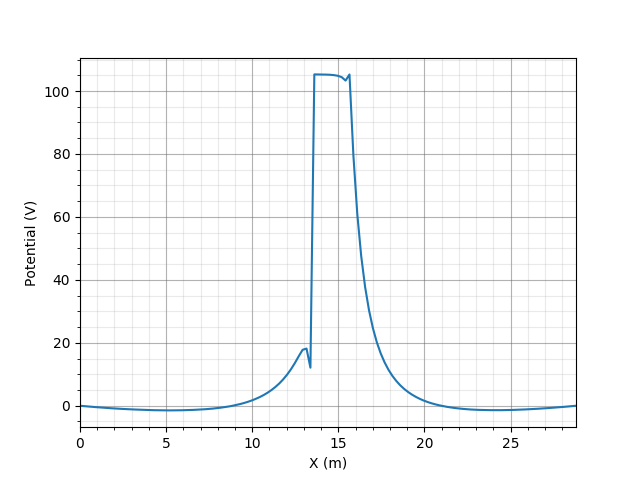
\includegraphics[width=\textwidth]{figures/MMO/BField/WB/L_BField_WB.png}
  \caption{Booms}
  \label{fig:L_BField_WB}
\end{subfigure}
\begin{subfigure}[b]{0.6\textwidth}
  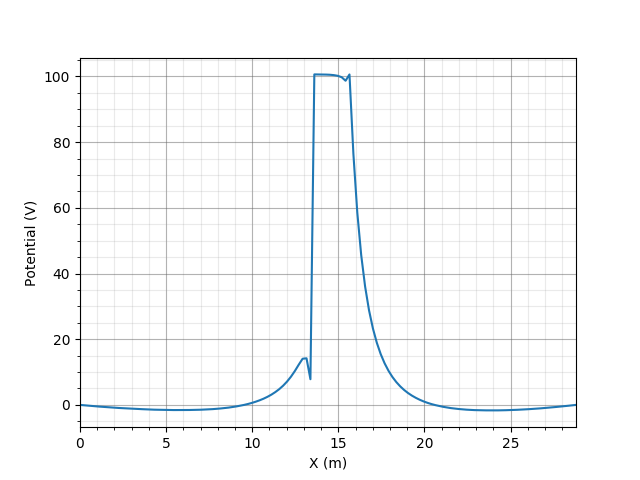
\includegraphics[width=\textwidth]{figures/MMO/BField/NB/L_BField_NB.png}
  \caption{Without booms}
  \label{fig:L_BField_NB}
\end{subfigure}
\label{fig:Line_BField}
\caption{Dummy text}
\end{figure}

%AVERAGE POTENTIAL ISOLINES XY
\begin{figure}[H]
  \begin{subfigure}[b]{0.6\textwidth}
    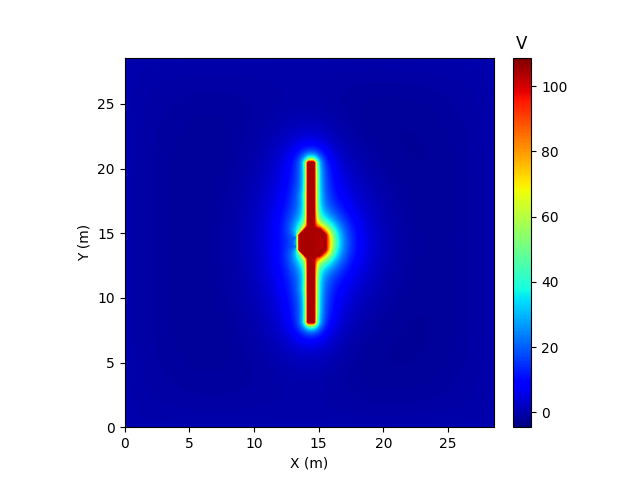
\includegraphics[width=\textwidth]{figures/MMO/BField/WB/P_BField_WB.png}
    \caption{Booms}
    \label{fig:P_BField_WB}
  \end{subfigure}
  \hfill
  \begin{subfigure}[b]{0.6\textwidth}
    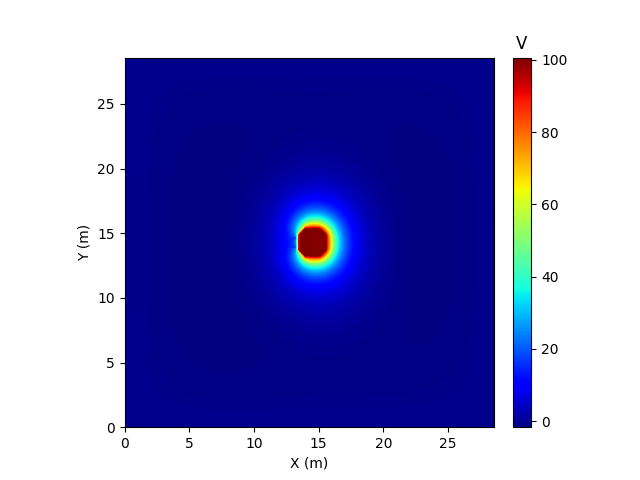
\includegraphics[width=\textwidth]{figures/MMO/BField/NB/P_BField_NB.png}
    \caption{Without booms}
    \label{fig:P_BField_NB}
  \end{subfigure}
  \label{fig:Pot_BField}
  \caption{Dummy text}
\end{figure}

%PARTICLE DENSITIES (rho_i and rho_e)
%RHO_I
\begin{figure}[H]
  \begin{subfigure}[b]{0.6\textwidth}
  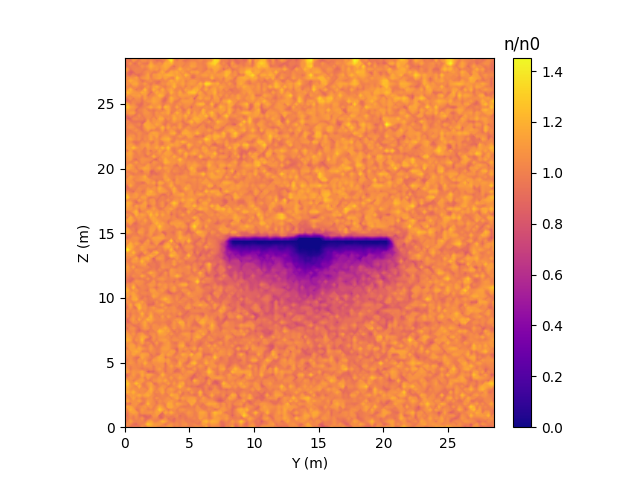
\includegraphics[width=\textwidth]{figures/MMO/BField/WB/I_BField_WB.png}
  \caption{Booms}
  \label{fig:I_BField_WB}
\end{subfigure}
\begin{subfigure}[b]{0.6\textwidth}
  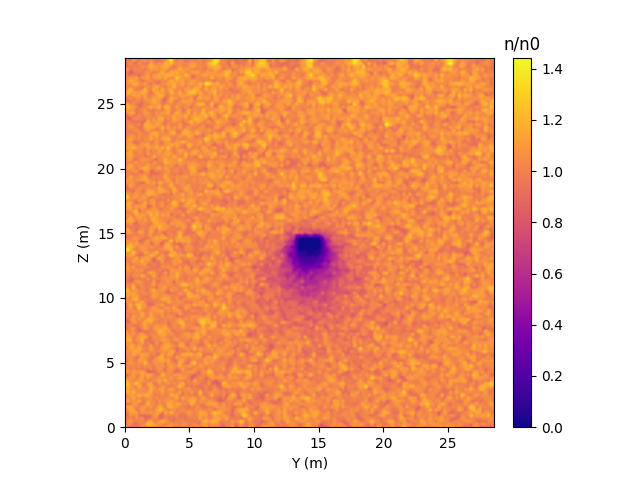
\includegraphics[width=\textwidth]{figures/MMO/BField/NB/I_BField_NB.png}
  \caption{Without booms}
  \label{fig:I_BField_NB}
\end{subfigure}
\label{fig:Ions_BField}
\caption{Dummy text}
\end{figure}

%RHO_E
\begin{figure}[H]
  \begin{subfigure}[b]{0.6\textwidth}
  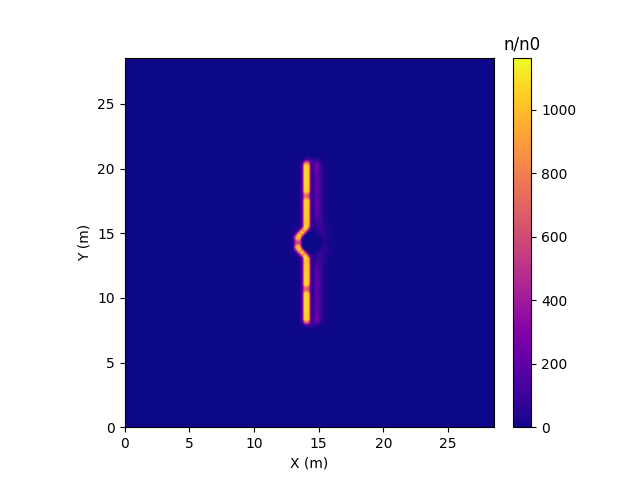
\includegraphics[width=\textwidth]{figures/MMO/BField/WB/E_BField_WB.png}
  \caption{Booms}
  \label{fig:E_BField_WB}
\end{subfigure}
\begin{subfigure}[b]{0.6\textwidth}
  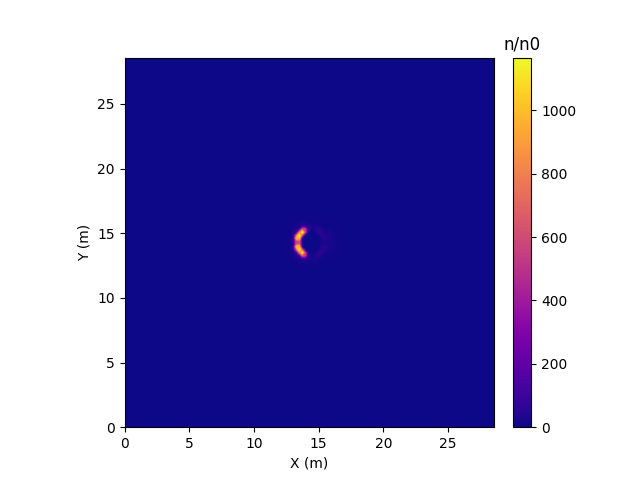
\includegraphics[width=\textwidth]{figures/MMO/BField/NB/E_BField_NB.png}
  \caption{Without booms}
  \label{fig:E_BField_NB}
\end{subfigure}
\label{fig:Elec_BField}
\caption{Dummy text}
\end{figure}

\section{Charging at different photoelectron temperatures}

%FLOATING POTENTIAL CONVERGENCE
\begin{figure}[H]
  \centering
  \begin{subfigure}[b]{0.75\textwidth}
  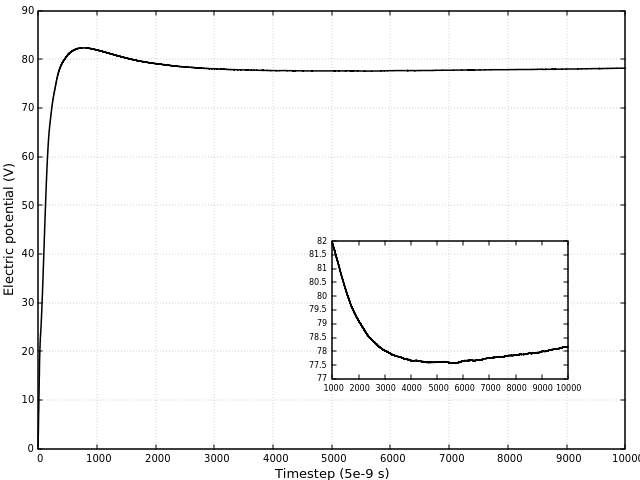
\includegraphics[width=\columnwidth]{figures/MMO/PHTemp/WB/C_PHTemp_WB.png}
  \caption{Booms}
  \label{fig:C_PHTemp_WB}
\end{subfigure}
\par\bigskip
\begin{subfigure}[b]{0.75\textwidth}
  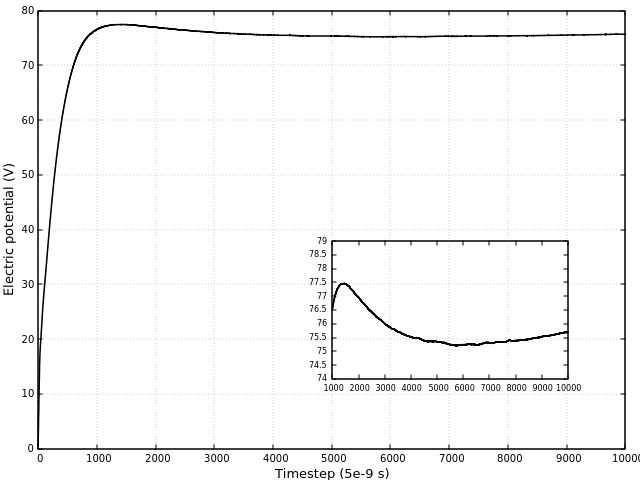
\includegraphics[width=\columnwidth]{figures/MMO/PHTemp/NB/C_PHTemp_NB.png}
  \caption{Without booms}
  \label{fig:C_PHTemp_NB}
\end{subfigure}
\label{fig:Conv_PHTemp}
\caption{Dummy text}
\end{figure}

%POTENTIAL THROUGH CENTER OF OBJECT
\begin{figure}[H]
  \begin{subfigure}[b]{0.6\textwidth}
  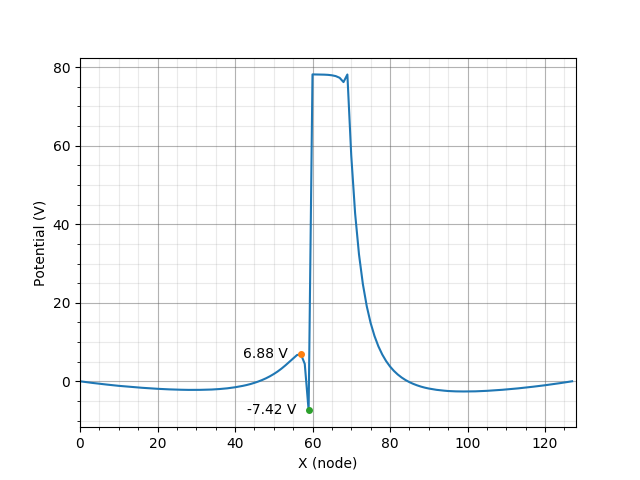
\includegraphics[width=\textwidth]{figures/MMO/PHTemp/WB/L_PHTemp_WB.png}
  \caption{Booms}
  \label{fig:L_PHTemp_WB}
\end{subfigure}
\begin{subfigure}[b]{0.6\textwidth}
  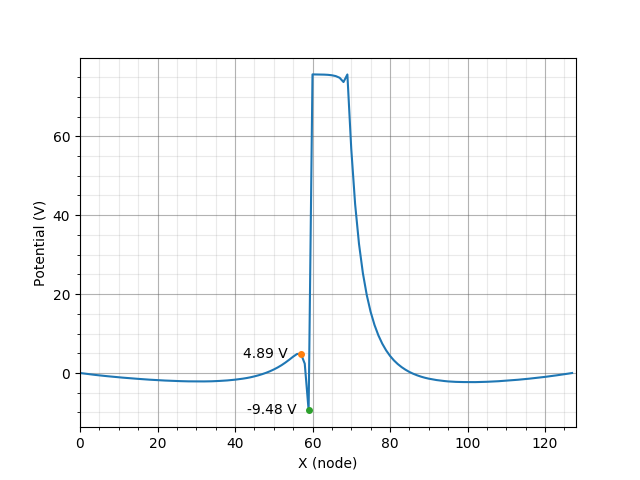
\includegraphics[width=\textwidth]{figures/MMO/PHTemp/NB/L_PHTemp_NB.png}
  \caption{Without booms}
  \label{fig:L_PHTemp_NB}
\end{subfigure}
\label{fig:Line_PHTemp}
\caption{Dummy text}
\end{figure}

%AVERAGE POTENTIAL ISOLINES XY
\begin{figure}[H]
  \begin{subfigure}[b]{0.6\textwidth}
    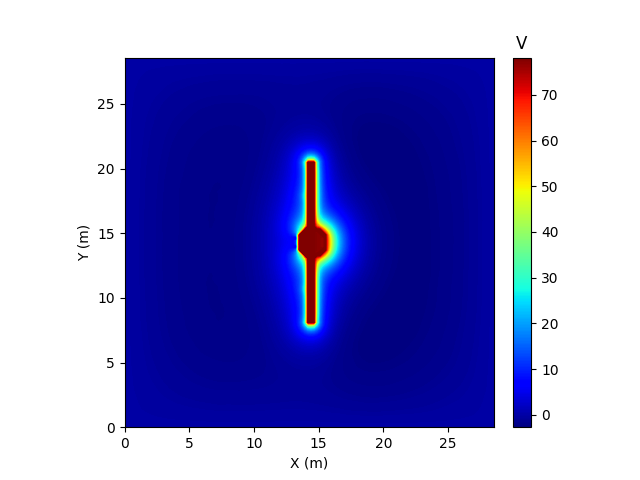
\includegraphics[width=\textwidth]{figures/MMO/PHTemp/WB/P_PHTemp_WB.png}
    \caption{Booms}
    \label{fig:P_PHTemp_WB}
  \end{subfigure}
  \hfill
  \begin{subfigure}[b]{0.6\textwidth}
    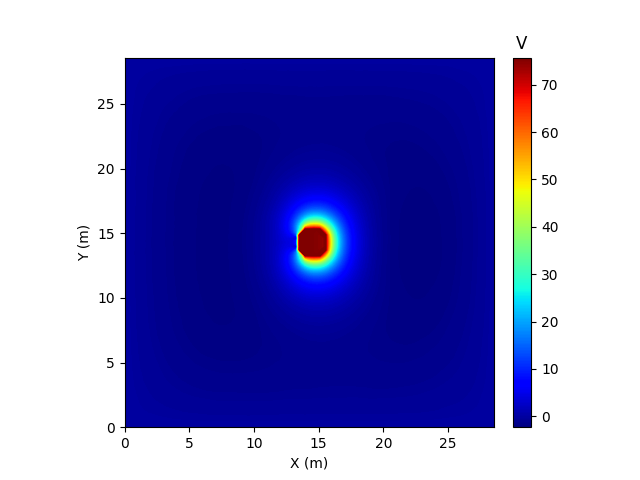
\includegraphics[width=\textwidth]{figures/MMO/PHTemp/NB/P_PHTemp_NB.png}
    \caption{Without booms}
    \label{fig:P_PHTemp_NB}
  \end{subfigure}
  \label{fig:Pot_PHTemp}
  \caption{Dummy text}
\end{figure}

%PARTICLE DENSITIES (rho_i and rho_e)
%RHO_I
\begin{figure}[H]
  \begin{subfigure}[b]{0.6\textwidth}
  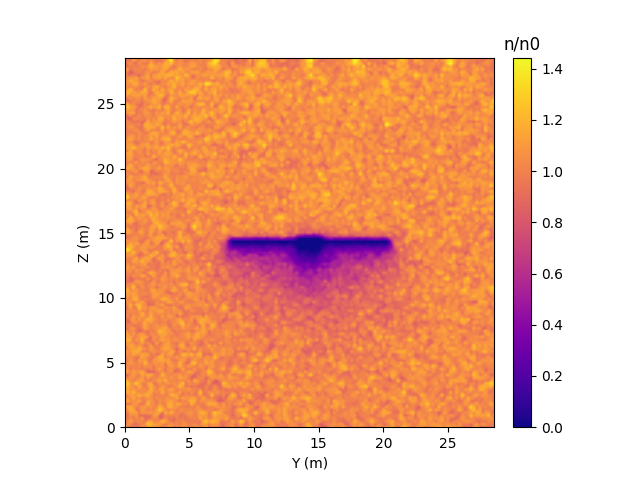
\includegraphics[width=\textwidth]{figures/MMO/PHTemp/WB/I_PHTemp_WB.png}
  \caption{Booms}
  \label{fig:I_PHTemp_WB}
\end{subfigure}
\begin{subfigure}[b]{0.6\textwidth}
  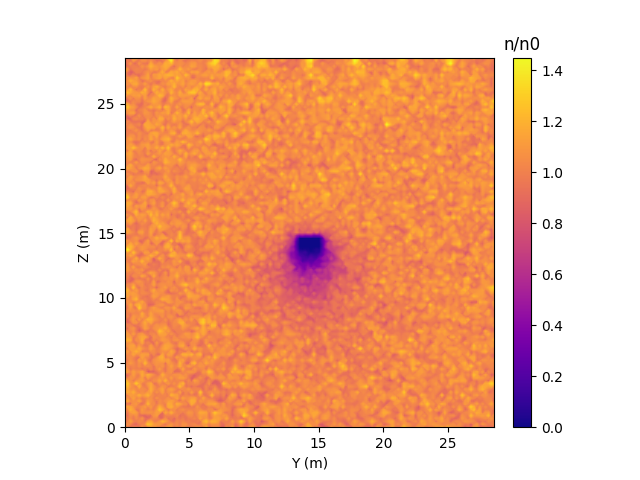
\includegraphics[width=\textwidth]{figures/MMO/PHTemp/NB/I_PHTemp_NB.png}
  \caption{Without booms}
  \label{fig:I_PHTemp_NB}
\end{subfigure}
\label{fig:Ions_PHTemp}
\caption{Dummy text}
\end{figure}

%RHO_E
\begin{figure}[H]
  \begin{subfigure}[b]{0.6\textwidth}
  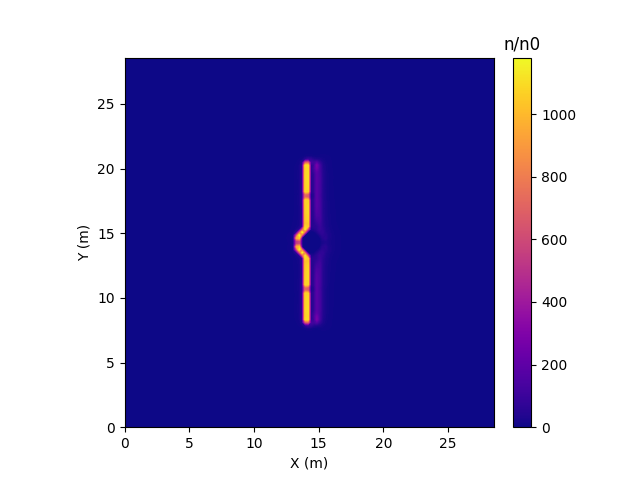
\includegraphics[width=\textwidth]{figures/MMO/PHTemp/WB/E_PHTemp_WB.png}
  \caption{Booms}
  \label{fig:E_PHTemp_WB}
\end{subfigure}
\begin{subfigure}[b]{0.6\textwidth}
  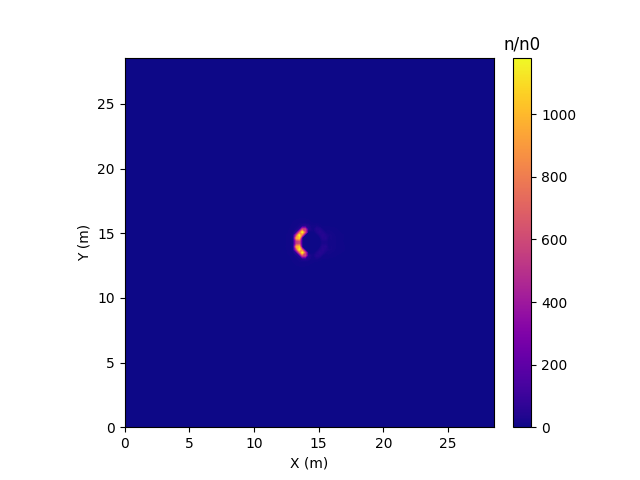
\includegraphics[width=\textwidth]{figures/MMO/PHTemp/NB/E_PHTemp_NB.png}
  \caption{Without booms}
  \label{fig:E_PHTemp_NB}
\end{subfigure}
\label{fig:Elec_PHTemp}
\caption{Dummy text}
\end{figure}